\documentclass[journal,12pt,twocolumn]{IEEEtran}
\usepackage{amsmath,amsfonts,amssymb,float,gvv,graphicx,enumitem,array,esint}
\bibliographystyle{IEEEtran}
\vspace{3cm}
\title{GATE 2021-EE-31}
\author{Pragnidhved Reddy\\EE23BTECH11050}
\date{}
\parindent 0px
\begin{document}
\maketitle
\newpage
\bigskip
\textbf{GATE 21 EE 31:}\\
The causal signal with z-transform $\frac{z^2}{(z-a)^{2}}$  is \\
\solution\\
Given z transform of the signal is $\frac{z^2}{(z-a)^{2}}$= $\left(\frac{1}{1-az^{-1}}\right)^2$\\
Let the signal be $x(n)$
\begin{align}
x(n)&=\mathcal{Z}^{-1}\left(\frac{1}{1-az^{-1}}\right)^2\\[6pt]
\left(\frac{1}{1-az^{-1}}\right)^2&\overset{Z}\longleftrightarrow (n+1)a^nu(n)\quad \abs{z}>\abs{a}\\[6pt] 
x(n)&=(n+1)a^n u(n)
\end{align}
$x(n)$ should be absolutely summable. Let s(n) be the sum till n terms. Then $s(\infty)$ should be a constant
\begin{align}
s(n)&=\sum_{m=0}^{n-1}x(n)\\
s(n)&=\sum_{m=0}^{n-1}(m+1)a^m\\
\label{eq:eq6_ee_31}
s(\infty)&=\sum_{m=0}^{\infty}(m+1)a^m\\
\label{eq:eq7_ee_31}
\frac{s(\infty)}{a}&=\sum_{m=0}^{\infty}(m+1)a^{m-1}
\end{align}
Subtract \eqref{eq:eq7_ee_31} from \eqref{eq:eq6_ee_31}
\begin{align}
s(\infty)\left(1-\frac{1}{a}\right)&=-\left(\frac{1}{a}\right)-\left(\sum_{m=0}^{\infty}a^{m}\right)\\
s(\infty)\left(\frac{a-1}{a}\right)&=-\left(\frac{1}{a}\right)-\left(\frac{1}{1-a}\right) \quad \abs{a}<1\\
s(\infty)&=\frac{1}{(a-1)^2}
\end{align}
Therefore, $\abs{a}<1$ for x(n) to be absolutely summable.
\begin{figure}[h!]
    \centering
    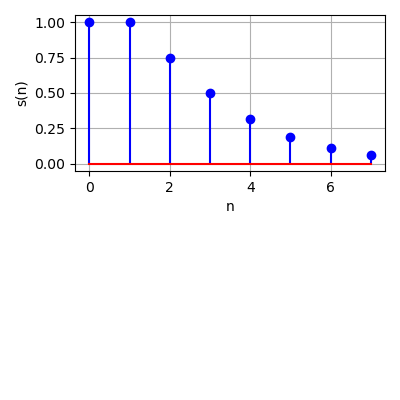
\includegraphics[width=\columnwidth]{figs/plot.png}
    \caption{graph of general term}
    \label{fig:1}
\end{figure}
\end{document}
